%%%% ijcai18.tex

%%%%%%%%%%%%% 1. Finish the scheduling model. I will have 8 pages then.         DONE
%%%%%%%%%%%%% 2. Finish the introduction. I will have 8.5 pages                 DONE
%%%%%%%%%%%%% 3. Finish the comparison with previous work, I will have 9 pages.
%%%%%%%%%%%%% 4. Finish the conclusion, I will have 9.25 pages.                 DONE
%%%%%%%%%%%%% 5. Expand the class effect and input size, then I will have 10.25 pages.
%%%%%%%%%%%%% 6. Add experiments on scheduling model, I will have 11.25 pages.




\typeout{IJCAI-18 Instructions for Authors}

\documentclass{article}
\pdfpagewidth=8.5in
\pdfpageheight=11in
\usepackage{sd}
\usepackage{bbm}
\usepackage{times}
\usepackage{xcolor}
\usepackage{soul}
\usepackage{comment}
\usepackage[utf8]{inputenc}
\usepackage[small]{caption}
\usepackage{latexsym} 
\usepackage{amsmath}
\usepackage{graphicx}
\usepackage{caption}
\usepackage{subcaption}
\usepackage{array}
\usepackage{amsmath}
\usepackage{amsfonts}
\usepackage{graphicx}
\usepackage[colorinlistoftodos]{todonotes}
\usepackage{algorithm}
\usepackage{algpseudocode}
\graphicspath{ {images/} }

\usepackage{geometry}
 \geometry{
 a4paper,
 total={210mm,297mm},
 left=20mm,
 right=20mm,
 top=20mm,
 bottom=20mm,
 }


\usepackage{graphicx,epstopdf}
\epstopdfsetup{update}
\DeclareGraphicsExtensions{.ps}
\epstopdfDeclareGraphicsRule{.ps}{pdf}{.pdf}{ps2pdf -dEPSCrop -dNOSAFER #1 \OutputFile}



\title{SMART: Runtime Support for Personalized AI}
\author{
Boyuan Feng, 
Yufei Ding
\\ 
Department of Computer Science \\
University of California, Santa Barbara \\
\{boyuan, yufeiding\}@cs.ucsb.edu
}
\setlength\titlebox{2.5in}

\begin{document}

\maketitle

\begin{abstract}
    TO BE ADDED
    % Our contribution contains three part:
    %   1. We explore different kind of specialization
    %   2. For simple model, we explore the effectiveness of retraining
    %   3. For complex model, we bring up a new method called probability layer, which could use run time distribution without retraining. The benefit could be 25\%.
    %   4. We bring up a automatic framework, which equips a pool of specialized models distilled effectively from a general, complex model. 
\end{abstract}

\section{Introduction}
Image classification and video processing are important areas due to their abundant applications in daily life. Robotics are desired to have ability in object recognition and provide different service to different people according to the ownership automatically without any human intervention. Mobile device, like AI-powered smart glasses, are desired to detect different types of objects, identify current environment by recognized objects, and give user real-time suggestion when it is necessary. All of these exciting applications are centered around image classification and introduce lots of attention to this area. In recent years, unprecedented advance has been made by using convolutional neural network (CNN). ResNet \cite{he2016deep}, a CNN architecture brought up by Microsoft on 2016, achieves top-5 error as 3.57\% on ImageNet, a prevalent benchmark for image classification with 1000 labels and 1.3 million graphs. This result is even better than what human can achieve, given the fact that reported average human top-5 error rate is 5.1\% \cite{russakovsky2015imagenet}. A popular perspective is to use CNN models on mobile devices and finally build technical armors just like Iron Man.

However, we still cannot do it yet due to the huge energy and memory consumption by CNN models. Table \ref{tab:compare} shows the summary of memory and computation of several prevalent networks. For training a CNN model from scratch, we generally need multiple GPUs running for several hours, sometimes even for weeks. In the other hand, several billion computations are needed in the inference for a single image. This is unacceptable on mobile device, a energy-restricted circumstance. To solve this problem, we bring up SMART, a runtime support for personalized AI, which could make use of environment, adjust the complexity of CNN models in the runtime, and choose feasible models according to current energy and memory budgets. Through deployment on a series of videos from Youtube, SMART shows its effectiveness by decreasing memory by xx times, and computation by xx times, while accuracy would be almost same or even higher. (EXPERIMENTS TO BE ADDED)


%Nowadays, convolutional neural network (CNN) shows incomparable advantage over other image classification algorithms. On the prevalent benchmark ImageNet \cite{imagenet_cvpr09}, a dataset with 1000 classes and 1.3 million images, the lowest top-5 error before the appearance of CNN models is 25.7\%, achieved by XRCE \cite{sanchez2011high}. Top-5 error means that the model gives the possibility of all classes given an image and we treat the prediction as correct if the true label is among the top-5 classes ranked by probability. On the appearance of the first CNN model on 2012, AlexNet \cite{NIPS2012_4824} achieves top-5 error rates of 17.0\%. Lately, K. Simonyan and A. Zisserman brought up VGGNet \cite{simonyan2014very}, which decrease the top-5 error further to 7.3\%. On 2015, Microsoft brought up ResNet \cite{he2016deep}, which achieves a top-5 error rate of 3.57\%. Considering that top-5 error that human can achieve is only 5.1\% \cite{russakovsky2015imagenet}, CNN has performed better than human and good enough for usage in daily life. 

\begin{figure} 
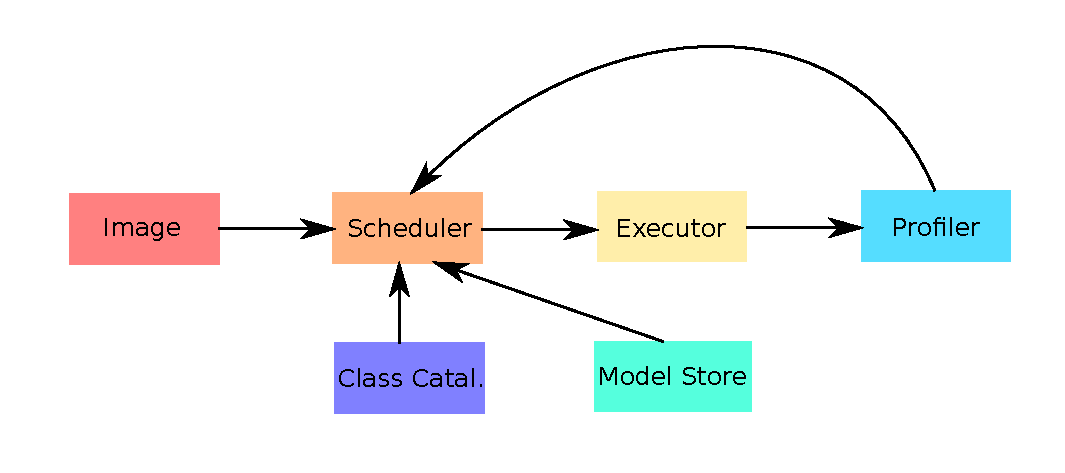
\includegraphics[scale=0.46]{Architecture.ps}
\caption{Overall architecture: This graph shows the overall architecture of SMART framework. The input are images. Every image will be forwarded into the scheduler. The scheduler first refers to the profiler and check whether there is a class skew. Then the scheduler will estimate the energy constraint for this image and choose the model with best accuracy given this energy constraint. The executor will follow the scheduler's decision and grasp the corresponding model from model store, which is a on-disk storage of previous train-ed models. Finally, the predicted value will be recorded by profiler for future usage.}
\label{fig:Architecture}
\end{figure}


%. Given the high accuracy that CNN models can achieve, the shortage that prevents CNN models from major deployment is energy and memory efficiency. Table \ref{tab:compare} shows the summary of memory and computation of several prevalent networks. For training a CNN model from scratch, we generally need several GPUs running for several hours, sometimes even for weeks. For the inference, we models generally need several billion computations. Due to the heaviness and cost of high-performance GPUs, we cannot equip mobile device with enough energy and computation power and we cannot always run the complex model. In other words, the energy and memory constrain are the important factors that cannot be avoided when we want to deploy powerful CNN models on mobile device. Since we have strong case in implementing DNNs on mobile phones and wearable devices, a natural question would arise: \textit{Can we use much less energy and memory resource to achieve a similar accuracy?} To solve this problem, we bring up SMART, a runtime support for personalized AI, which could make use of environment, adjust the complexity of CNN models in the runtime, and choose feasible models according to current energy and memory budgets. Through deployment on a series of videos from Youtube, SMART shows its effectiveness by decreasing memory by xx times, and computation by xx times, while accuracy would be almost same or even higher. (EXPERIMENTS TO BE ADDED)

\begin{comment}
\begin{figure*}
\centering
\begin{subfigure}{.2\textwidth}
  \centering
  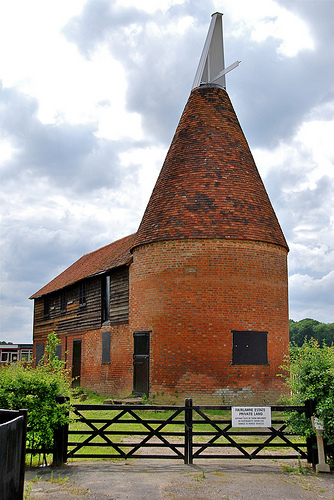
\includegraphics[scale=0.2]{classTypeExample1.jpg}
  \caption{House}
\end{subfigure}%
\begin{subfigure}{.2\textwidth}
  \centering
  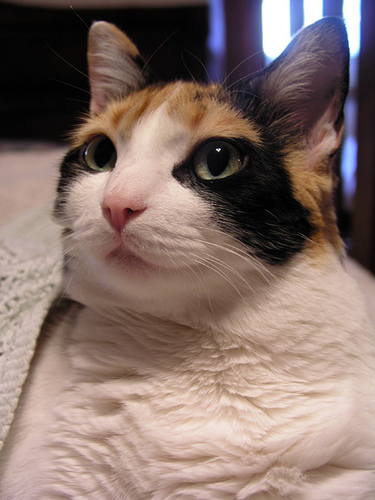
\includegraphics[scale=0.28]{classTypeExample2.jpg}
  \caption{Cat}
\end{subfigure}%
\begin{subfigure}{.2\textwidth}
  \centering
  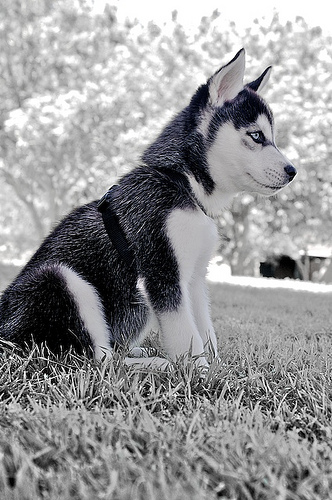
\includegraphics[scale=0.2]{classTypeExample3.jpg}
  \caption{Dog}
\end{subfigure}%
\begin{subfigure}{.2\textwidth}
  \centering
  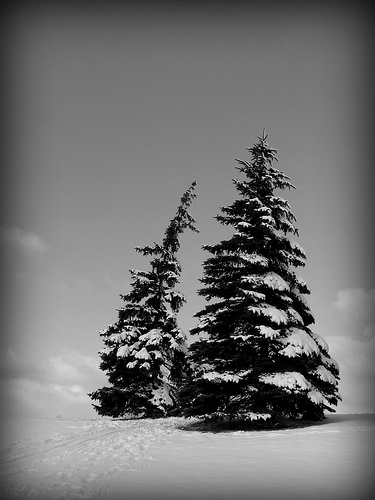
\includegraphics[scale=0.2]{classTypeExample4.jpg}
  \caption{Tree}
\end{subfigure}
\begin{subfigure}{.2\textwidth}
  \centering
  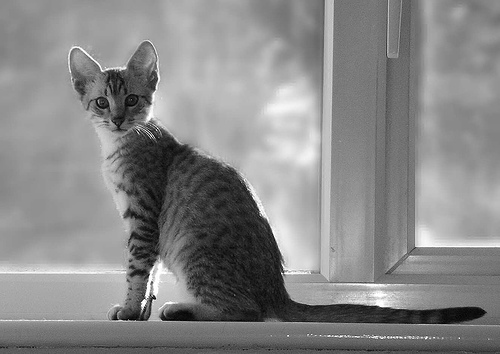
\includegraphics[scale=0.2]{classTypeExample5.jpg}
  \caption{Egyptian Cat}
\end{subfigure}
\begin{subfigure}{.2\textwidth}
  \centering
  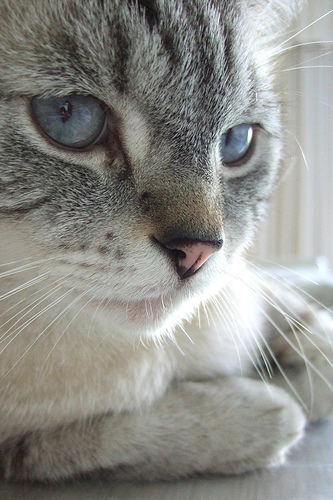
\includegraphics[scale=0.22]{classTypeExample6.jpg}
  \caption{Kitty Cat}
\end{subfigure}
\begin{subfigure}{.2\textwidth}
  \centering
  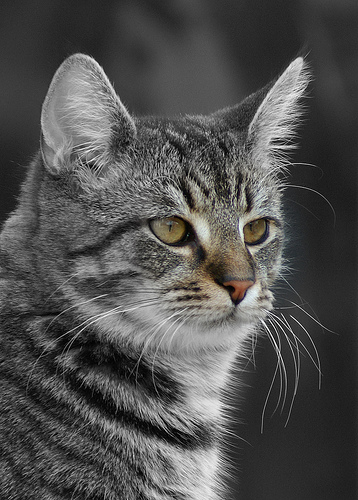
\includegraphics[scale=0.3]{classTypeExample7.jpg}
  \caption{Tiger Cat}
\end{subfigure}
\begin{subfigure}{.2\textwidth}
  \centering
  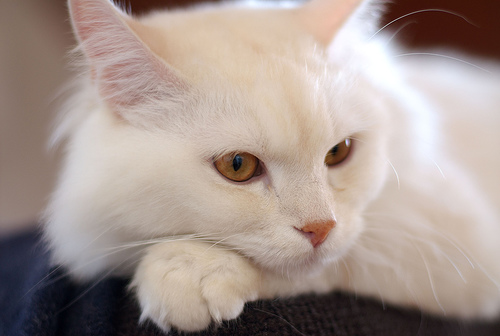
\includegraphics[scale=0.2]{classTypeExample8.jpg}
  \caption{Angora Cat}
\end{subfigure}


\caption{This set of images shows the class effect. The images in the first row shows objects in four coarse-grained labels: house, cat, dog, and tree. The second row represents different species of cats, Egyptian cat, Kitty cat, Tiger cat, and Angora cat, which are more fine-grained labels. All of these images come from ImageNet. Intuitively, it is much easier to distinguish house, cat, dog, and tree than classifying four cat species, since different cat species share more common features and varies only in subtle features like eye colors, fur colors or coat patterns. To learn these subtle features a more complicated model is needed while a much simpler model is enough for differentiating house, cat, dog, and tree. }
\label{fig:classEffect}
\end{figure*}
\end{comment}

One phenomenon that we use extensively is the class skew, which includes reduction in number of classes and class effect. Reducing number of classes has been mentioned in previous papers \cite{han2016mcdnn} \cite{shen2016fast} (MORE CITATION?) and shows benefit on increasing accuracy and reducing resource consumption. (MORE EXPERIMENT RESULTS) However, existing papers only discussed number of classes and does not pay attention to class effect. Through a series of experiments, we found that, even if the number of classes remains unchanged, what the selected classes represent also plays an important role in classification process and leads to dramatically different accuracy on the same CNN architecture. Figure \ref{fig:classEffect} shows that this observation follows our intuition since classifying house, cat, dog, and tree is much easier than distinguishing four different cat species even if the number of classes remain unchanged. By using this class effect, we can simplify models with guidance from similarity between classes and use less energy to achieve same accuracy. Naturally, a semantic tree representing closeness of labels in semantic has been discussed to model class effect. However, the way that algorithms found similarity is largely different from human's feeling. Thus we proposed a more advanced quantitative method, \textit{QuantClosenesses}, by mimicing the thinking process of CNN models. 

The improvement on accuracy brought in by class skew provides the space for model simplification. There are two difference between our work and existing papers (CITATION). First, while all of existing papers only discuss ruducing number of classes and number of layers, we introduce varying input size and distillation into this area. The interaction between optimization methods and class effect is also discussed and measured in quantitative ways. The second difference, which is more intrinsic, is how we search candidate models: we use guided search while existing papers use exhaustive search. Previous papers would search all possible combination of optimization methods exhaustively through trying every optimized model one by one without any theory guidance. This exhaustive method is unacceptable in practice since there are mind-bogglingly huge numbers of optimized models. Instead we bring up guided search to give estimation of most suitable models and reduce work in choosing-model process. We will have a mapping from groups of classes to suggested models, including every detail in the model such as input size, number of layers, and even number of nodes in each layer.

To use class skew and optimization methods, retraining the model is unavoidable. Retraining is time-consuming and needs lots of computation power and energy, sometimes even very tricky and need experts to fine-tune the model. GoogLeNet \cite{szegedy2015going} needs several high-end GPUs and consume a week to converge, which is infeasible in both time and resource to retrain in the runtime. VGGNet \cite{simonyan2014very} needs carefully weights initialization and multi-peiord training, which means train a shallow model first, use the trained weights to initialize a deeper model, and train this deeper model further. This manually training process is hard to be done automatically, which becomes obstacle for the runtime retrain. Three methods targetting different energy budget are discussed in order to solve these problems. If there are enough energy, we can retrain the last few layers. With little energy, we can use an extra layer, called probability layer, to use runtime distribution without any retrain. For the class skew appearing frequently, we can cold-train the model and save it on disk for future usage. Section 4 will discuss retraining in detail.

Finally, we will bring up a runtime supporting framework, called SMART. Figure \ref{fig:Architecture} provides an overview of the architecture. An image will be sent to scheduler as input. Scheduler is an optimization algorithm to choose the model automatically according to current available resource. To support the decision, the scheduler will refer to model store for available pre-trained models and refer to class catalog for better understanding of difficulty in distinguish target classes. With these information, the scheduler will calculate the available energy budget and choose the best model to maximize the accuracy. Then the chosen model will be forwarded to executor and executor will load and execute that model. The predicted value will be recorded by profiler for future decision. The architecture will be covered in section 5.

\begin{table}[!th]
    \centering
    \begin{tabular}{|l|c|c|c|c|}
        \hline
        \multicolumn{1}{|c|}{Model Name} & Parameter& Computation \\
        \hline
        AlexNet &  60M & 1.5B \\
        VGG16   & 138M &  30B \\
        ResNet  &  60M &  23B \\
        \hline
    \end{tabular}
    \vspace{1em}
    \caption{Summary of parameters and computation usage}
    \label{tab:compare}
\end{table}


%\begin{figure*}
%\centering
%  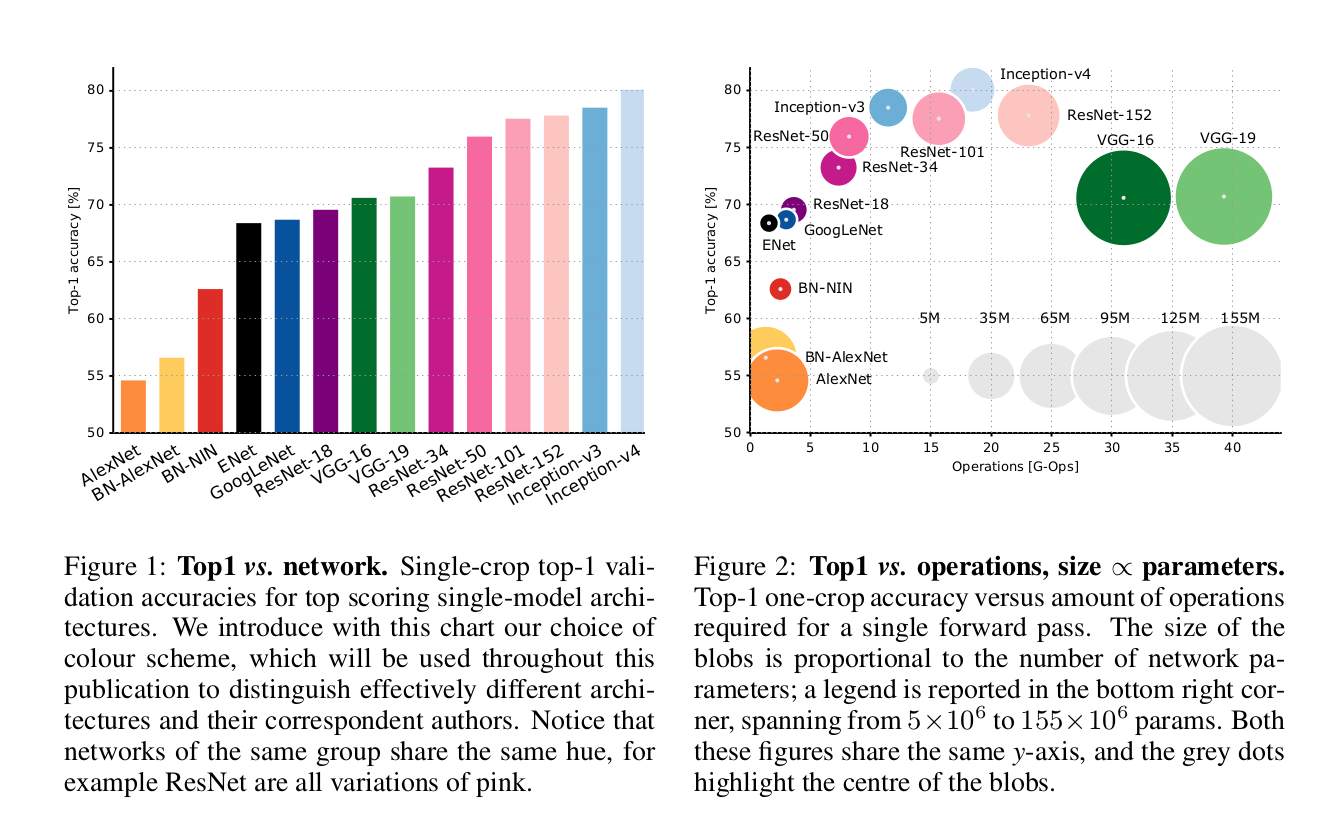
\includegraphics[scale=0.4]{resourceUsage.png}
%\caption{Summary of memory and computation usage by different architectures}
%\label{fig:resourceUsage}
%\end{figure*}

In summary, our contribution remains in three parts.
\begin{enumerate}
  \item Discuss the effect of class skew on model accuracy.
  \item  Discussed the optimization methods tailored for class skew and how to retrain a model. We bring up probability layer to make use of runtime class distribution without retrain. 
  \item  Bring up a runtime supporting architecture, SMART, for making use of run time class skew automatically according to available energy and existing models.
\end{enumerate}

\iffalse
\begin{table*}[!th]
    \centering
    \begin{tabular}{l|c|c}
        \hline
        \multicolumn{1}{c|}{Component} & Percentage of Total Computation  & Percentage of Total Memory \\
        conv3-64 & 0.56\% & 0.00\% \\
        conv3-64 & 11.95\% & 0.03\% \\
        \hline
        conv3-128 & 5.98\% & 0.05\% \\
        conv3-128 & 11.95\% & 0.11\% \\
        \hline
        conv3-256 & 5.98\% & 0.21\% \\
        conv3-256 & 11.95\% & 0.43\% \\
        conv3-256 & 11.95\% & 0.43\% \\
        \hline
        conv3-512 & 5.98\% & 0.85\% \\
        conv3-512 & 11.95\% & 1.71\% \\
        conv3-512 & 11.95\% & 1.71\% \\
        \hline
        conv3-512 & 2.99\% & 1.71\% \\
        conv3-512 & 2.99\% & 1.71\% \\
        conv3-512 & 2.99\% & 1.71\% \\
        \hline
        FC-4096   & 0.66\% & 74.28\% \\
        FC-4096   & 0.11\% & 12.13\% \\
        FC-1000   & 0.03\% & 2.96\% \\
        \hline
        Non-FC Layers & 99.20\% & 10.64\% \\
        \hline
        FC Layers & 0.80\% & 89.36\% \\
    \end{tabular}
    \vspace{1em}
    \caption{Memory and computation usage of VGG16}
    \label{tab:distribution}
\end{table*}
\fi


\section{Impact of Class on Accuracy}


\subsection{Specialization}

One phenomenon that we uses extensively in SMART is class skew. Actually, in real life, the appearance of classes is not random. A class tends to appear frequently in a time period, disappears later, and appear for a long time period again in the future. And a cluster of classes tends to appear together and sometimes we can inference that class B is nearby if we see class A. For example, in office, we expect to only see our collaborators and we will not see our family members, while generally only family members will appear in home and collaborators are not expected to appear in our house. If our model detects that many collaborators appear, a reasonable guess would be that we can only see people out of collaborators. In this case, although we have a complex model that can recognize both collaborators and family members, we need a simpler model which could recognize collaborators and do not need the full model ability for family members. This class skew gives us chance to simplify our model and use less resource. A good result is that class skew could automatically lead to improvement on accuracy without any change in model. We will discuss these environment and benefit in section 2. 


\subsubsection{What is Specialization}
When we train a model, we would want a general one, since our model should be able to handle as many as cases. However, when we actually run our model in daily life, we do not need our model to be that powerful at all the times, since our life have some context and patterns. For example, we have a strong model focusing on face recognition. This model knows all the people we would meet in our whole life, where the number is around 10000. However, if we go for vacation with our family members, we will only need to recognize less than 10 people in this trip. Thus in this trip, we only need to run a smaller model which could only recognize 10 peoples. This smaller model is called a \textit{specialized model}.

\subsubsection{What is the benefit of specialization}
One benefit is reducing memory usage. When we run the original model which could recognize 10000 people, the last fully connected layer would have 10000 classes and the number of parameters in this layer is $10000 \times n$, where $n$ is the length of input vector. If we use the specialized model, which only have 10 classes, instead of the general one, the number of parameters in the fully connected layer is $10 \times n$, which is $100$ times less than the original model.
Another benefit is the improvement in accuracy.From the point view of random guess, if we need to guess from 1000 classes randomly, the accuracy would be $0.1\%$. If we need to guess from 10 classes, the accuracy would be $10\%$. In other words, only using this single extra information, also known as \textit{temporal locality}, we can increase accuracy by 100 times. This gives specialization incredible potential in compressing models while increase accuracy.

\subsubsection{How can we implement Specialization}
The methods of specialization mainly contains three parts.
\begin{enumerate}
    \item In the fully connected layer, reduce number of output channels. For example, if we have a network pre-trained on ImageNet, which targets for 1000 classes, and only ten classes occurs frequently now, the number of output channels could be reduced from 1000 to 10. Using this method, we can reduce the memory usage by 100 times while keeping accuracy or even increase accuracy dramatically. This could be easily done by keep the parameters in the Non-FC layers unchanged, reduce the output vector of FC layers to 10, and only re-train the FC connected layers. Since we don't retrain the convolutional layers, we can save lots of computations.
    
    
    \item We can reduce number of convolutional layers, which could reduce number of computations proportionally.
    
    \item For every chunk of convolutional layers, delete one layer per chunk, instead of delete a whole chunk. Every type of convolutional layer may have some special usage. To give more freedom in our model, we should use more types of convolutional layers instead of just replicating same layer multiple times.
    
    \item Every time when we retrain a specialized model, we can record this model on disk. Since we live in the similar environment everyday, we can use this specialized model directly and do not need re-train it. This method makes sense, since every user have same usage patterns. For instance, they might meet the same group of people in office, same family members at home, and similar friends in habit groups. Along this way, we can use specialization without re-training, after the users used our application for a few days. Actually, other people who appears seldom in our life generally are the people who we do not need to recognize. Gradually, we may use this directory of specialized models to replace the original model totally.
\end{enumerate}
In the process of re-training specialized models, a rule proved by experiments is that we should keep at least two fully connected layers, while we can reduce the number of predicted classes as low as we want.


\subsubsection{When should we implement Specialization}
We will use a background process to record the distribution of classes, which is called $P_{underlying}$. Before we actually run our model, if we have a pre-knowledge about the distribution of classes, we can use it directly as the pre-defined distribution; if we do not have any pre-knowledge, we can assign equal probability to every class. In the process of classifying images, we can record the predicted class and keep updating the distribution $P_{underlying}$ by
\begin{equation}
    P_{underlying}(X = j) = \frac{num(j)+  \mathbbm{1}\{i = j\} }{totalNum + 1}
\end{equation}
, where num(j) is the appearance number of class j in recent 30 minutes, totalNum is the number of images that has been processed in recent 30 minutes, and $\mathbbm{1}\{i = j\}$ is the indicator function such that
\begin{equation}
  \mathbbm{1}\{i = j\}=\begin{cases}
    1, & \text{if $i==j$}.\\
    0, & \text{otherwise}.
  \end{cases}
\end{equation}

If we find that 10 classes accounts for 80\% images, we can re-train the specialized model and use this specialized model to classify images. As the distribution $P_{underlying}$ starts to show that these 10 classes occupy less than 80\% images, we will use the general model instead, and keep this specialized model on disk. When we confront the same condition again, we can pull this recorded specialized model from disk directly. 


\subsection{Class Effect}
Besides reduction of class numbers, we found the choice of classes also have tremendous impact on model accuracy. Even if we keep the number of nodes in the softmax layer, the accuracy could change dramatically due to the choice of different set of classes. For example, it would be easier to predict from aquatic mammals, flowers, household furniture, insects, and people, than predict from any finer subsets of each of these classes, like "baby, boy, girl, man, woman" or "bee, beetle, butterfly, caterpillar, cockroach". Intuitively, the difference between people and insects is much obvious than the difference between man and woman. If CNN model just want to distinguish people and insects, it only need to learn some low level features like the body shape. In contrast, if a CNN model need to predict from man and woman, the model might need to learn low level features such as body shape as well as complex features, like hairstyle, etc.

To support our conclusion, we conduct several experiments on CIFAR100 using a simple model with 4 convolutional layers and 3 fully connected layers. CIFAR100 is a dataset of graphs, with 20 coarse labels and 100 fine labels. Every graph has a coarse label and a fine label simultaneously. For every coarse label, there are 5 corresponding fine labels, which are more accurate descriptions. For example, "people" is a coarse label, and the 5 corresponding fine lables are "baby, boy, girl, man and woman" from "people" label. 

If we use the model to predict from quatic mammals, flowers, household furniture, insects, and people, which are 5 coarse labels in CIFAR100, the accuracy is 75\%. However, if we use finer labels inside each of these coarse labels, like "baby, boy, girl, man and woman" from "people" label, or "beaver, dolphin, otter, seal, whale" from "aquatic mammals" label, the accuracy would decrease dramatically to 55\%, even if we have changed nothing with number of classes in the softmax layer and the model architecture.

(HERE)How can we measure the closeness between classes? We will use the output of softmax layer in denseNet and. In detail, since denseNet \cite{huang2017densely} has achieved 5.29\% top-5 test accuracy on 

The naive method would be using closeness in semantics, like the tree-structured storage of images in ImageNet \cite{imagenet_cvpr09}. In a tree-structured storage, images will be grouped by labels and labels will be indexed like a tree according to their similarity in semantics. For example, the root might be mammal and has two children: dog and cat. Under the cat node, there are some children and each children node represents a cat species. This method does not work very well since there is a discrepancy between how human and deep learning models define classes. For human, we categorize objects from various aspects: appearance, functionality, ..., whereas most deep learning models like CNNs only focus on the appearance of an object, i.e.,  its 2D mapping. Instead, we introduces a new concept \textit{QuantClosenesses}, which fits better for CNN models in the task of recognization.



\section{Optimization Methods}
The improvement in accuracy brought in by class skew provides the space for model simplification. In other words, even if we simplify a model dramatically and use much less resource, we can still achieve a similar accuracy with the original full model. Existing model optimization methods (Reference TO BE ADDED) does not make use of the class skew and cannot exploit thoroughly the space introduced by class skew. Thus we explore a series of class-skew related optimization methods, including reducing input size, number of nodes in softmax layer, number of layers, and distillation. Through reducing input size, we can reduce computation by 16 times while keep the accuracy unchanged (Experiments TO BE ADDED). These optimization methods will be discussed in section 3.

\subsection{Input Size}
We also found that input size has influence on model accuracy. With the same model on CIFAR100, if we reduce the input size from 32*32 to 16*16 and further to 8*8, the accuracy will only decrease from 25\% to 23\% to 21\%, in the mean time the computation and memory cost has decreased by 4 and 16 times, respectively. This is a trade-off between model accuracy and resource.



\subsection{Distillation}
\subsubsection{What is Distillation and What is the benefit of distillation}
Large models with higher accuracy would contain more information than smaller models. When we find a chance for specializaion, we need to re-train a model for this specialized datasets. If we reduce the number of convolutional layers, we need to retrain the model from beginning. This is good. However, \textit{can we make use of the learned information in large models when we re-train the smaller model?}  One method is distillation \cite{hinton2015distilling}. Distillation means that we can treat large model as teacher and small model as student. Instead of train the student model directly on the original datasets with a vector of only 0-1, we can train the student model to mimic the logits of large model, which indicates how strongly the teacher model believes that this image belongs to this specific class. And hopefully the student model can learn more information from the teacher and achieve a higher accuracy. 

\subsubsection{How can we implement distillation}
Originally, when we train a model, we would define the loss function as 
\begin{equation}
    loss = - \sum_{i} y_i \cdot log(Y_i)
\end{equation}
, where $Y_i$ is the predicted value, and $y_i$ is the true value. \cite{hinton2015distilling} brings up a new loss function
\begin{equation}
    loss = 0.2 \cdot \sum_{i} y_i \cdot log(Y_i) + 0.8 \cdot \sum_{i} y_i \cdot log(Z_i)
\end{equation}
, where $Y_i$ is the calculated value, $y_i$ is the true value, $Z_i$ is the value calculated by the teacher model.

However, we still need a few modification to implement distillation in our case. Since in the specialization, each time we will have a specialized dataset which contains much less number of classes than the original dataset. But the length of $y_i$ and $Z_i$ is same as the original dataset and much larger than the number of classes in the specialized dataset. To solve this problem, we have the following methods.
\begin{enumerate}
    \item If we choose a subset $A$ out of all the classes as the specialized datasets, we will truncate and only use the indices in $y_i$ and $Z_i$ corresponding to $A$ in distillation.
    \item Use 
        \begin{equation}
            Y_{i}^{'} = \frac{0.9*Y_i}{\sum_{i \in A} Y_i}, i \in A
        \end{equation}    
\end{enumerate}



\subsubsection{When should we implement distillation}
Two ideas.
\begin{enumerate}
    \item For any specialization mentioned in last section, we can use distillation to improve the accuracy by 5\%.
    \item Distillation may works badly on some specialized models. Thus we should collect a catalog of specialized models which are good suits for distillation beforehand.
\end{enumerate}


\subsection{Reducing number of nodes in the softmax layer}



Nowadays, we have many deep networks which achieves incredibly high accuracy on several benchmarks, like CIFAR10, CIFAR100, and ImageNet. Keep these network in hands, our target is to simplify these networks, while keep accuracy. To discuss our methods thoroughly, we will use VGG16 \cite{simonyan2014very} as the object throughout this section.
In Table 2 (TABLE2 DELETED), we exhibit the memory and computation usage of VGG16 layer by layer. We can find that 99.20\% computation is used by convolutional layers, and computation usage is proportional to the number of convolutional layers. For the memory usage, 89.36\% is used by fully connected layers. The fully connected layer could be represented by a linear transformation
\begin{equation}
Y = M \times X    
\end{equation}
, where $Y$ is the output vector with length $m$, $X$ is input vector with length $n$, and $M$ is a $m \times n$ matrix. The memory usage of fully connected layers only exist in the matrix $M$, which is proportional to $m$ and $n$. Basically, the idea is to reduce computation usage by using less number of convolutional layers, and reduce memory usage by reducing the length of input and output vectors.


\subsection{Reduce number of layers}


\subsection{Interaction between class effect and optimization methods}

\section{Important factor in real life usage: Retrain}

\subsection{Repeated patterns in daily life and cold retrain}
Argue that same environment will appear again and again in daily life to support the argument that we can cold-train the model and save the trained model on disk to use in the following day. Save retrained, specialized models on disk for usage in the future!!! Disk is more cheap and we do not need to worry too much. This is an example to exchange speed and memory with disk space.

\textit{Experiments: use Youtube videos to show repeated patterns in daily life}

\subsection{Retrain the last few layers}
According to MCDNN, we can only retrain the last few layers. Retarget.


\subsection{Probability Layer}
\subsubsection{What is Probability Layer and What is the benefit of Probability Layer}
Previously, if we want to use the context information, we need to reduce the number of nodes in the final layer and retrain the neural network. It is hard to retrain model during run time, since retraining is a slow process, especially when we are using large models. It is also hard to cold retrain the model, since the point of retraining is to use the runtime distribution and we do not know this distribution beforehand. It is also unfeasible to cold retrain all the possible specialized models, since the number of all combinations is extremely huge. For example, if we choose 10 classes out of 100, the total number of combinations would be $\frac{100!}{10! \cdot 90!} = 1.73*10^{13}$. In short, retraining models is an obstacle for using specialization efficiently. To solve this problem, we bring up the probability layer which enables us to use runtime distribution without retraining. 

\subsubsection{How to implement probability layer}
As we all know, the last layer of CNN model would be the softmax layer. The output of the softmax layer is a vector $(p_1, p_2, ..., p_n)$, where $n$ is the number of nodes in the softmax layer, i.e. the number of classes that the CNN model wants to predict from. Also, $p_1$, ..., $p_n$ is a series of numbers between $0$ and $1$. Thus we would treat $p_i$ as the probability that indicates how likely an image may belong to a specific class $i$. The main idea of probability layer is to add a constant to classes that is more likely to be the true label according to the runtime distribution. For example, if the runtime distribution shows that only the first 10 out of 100 classes could appear in a context, the probability layer will add a constant to $p_1$, ..., $p_{10}$, the predicted probability of these 10 classes. In other word, in this case, the probability layer is $(c, c, c, c, c, c, c, c, c, c, 0, 0, ..., 0)$, where $c$ is a constant between $0$ and $1$ and the output of the probability layer is $(p_1 + c, p_2 + c, ..., p_{10}+c, p_{11}, ..., p_{99})$. Here we treat $c$ as a hyper-parameter. The larger the c is, the stronger confidence we have in runtime distribution.

\subsubsection{Good results for probability layer}
A series of experiments on various kind of specialized datasets have shown the effectiveness of probability layer. CIFAR100 is a prevalent benchmark for various kind of CNN models, which has 100 classes, a training dataset with 500 images per class, and a testing dataset with 100 images per class. To mimic the runtime distribution, we generate a specialized dataset manually. For example, in generation of a specialized dataset with 80\% data skew and 10 domain classes, we would use 1000 images from the testing dataset according to these 10 domain classes, and randomly select 250 images from other classes. We trained the model on original CIFAR100 training dataset and test the model on various kind of specialized datasets with different number of domain classes and selection of domain classes. We also take into account that the selection of domain classes because the choice of labels have strong effect on the test accuracy, even if we keep the number of domain classes unchanged. Actually some classes are easier to classify than others. To eliminate this random effect, we will choose different groups of labels for each number of domain classes.

Figure \ref{fig:ProbabilityLayer} summarizes the results. As a benchmark, the test accuracy on the CIFAR100 testing dataset without probability layer is 73.74\%. If the number of domain classes is 2 and we choose the label 0 and 1, the accuracy without probability layer is 88.12\%. The difference between specialized testing accuracy 88.12\% and the overall accuracy 73.74\% is due to selection of classes. If we change the label pair from (0,1) to (3,5), the accuracy would also change from 88.12\% to 61.39\%. However, in both case, the accuracy with probability layer are 98.51\% and 99.01\%, which performs very well consistently. 

Then we increase the number of domain classes from 2 to 5 and choose domain classes as 0 to 4 and 5 to 9 respectively. This time, the effectiveness of selection of domain classes appears again. If we set domain classes as 0 to 4, the accuracy without probability layer would be 66.33\%. If we set domain classes as 5 to 9, the accuracy would be 81.06\%. The accuracy with probability layer in these two cases would be 93.03\% and 97.01\% respectively. The benefit of probability layer are 26.70\% and 15.95\% respectively.

When we increase the number of domain classes further to 10, the effectiveness of probability layer would still be dramatic. We choose 0 to 9, 10 to 19, 20 to 29 as domain classes. The accuracy without probability layer would be 75.35\%, 67.16\%, and 75.84\%. The accuracy with probability layer would be 94.21\%, 91.41\%, and 92.22\%. The benefits are 18.86\%, 24.26\%, and 16.38\%.

To explore the interaction between probability layer and number of domain classes, we increase the number of domain classes gradually from 2 to 100. The benefit disappears gracefully. When number of domain classes is less than 20, the benefit are above 18\%. Even if we have 40 domain classes, the benefit is still around 10\%. When there are 60 classes, there are 5\% benefit. Since we do not need retrain, these benefit are almost free. We do not need extra memory or energy and we have not introduced any extra latency. The only thing that we need is the run time distribution, which could be collected easily through an in-memory record.


\begin{figure}
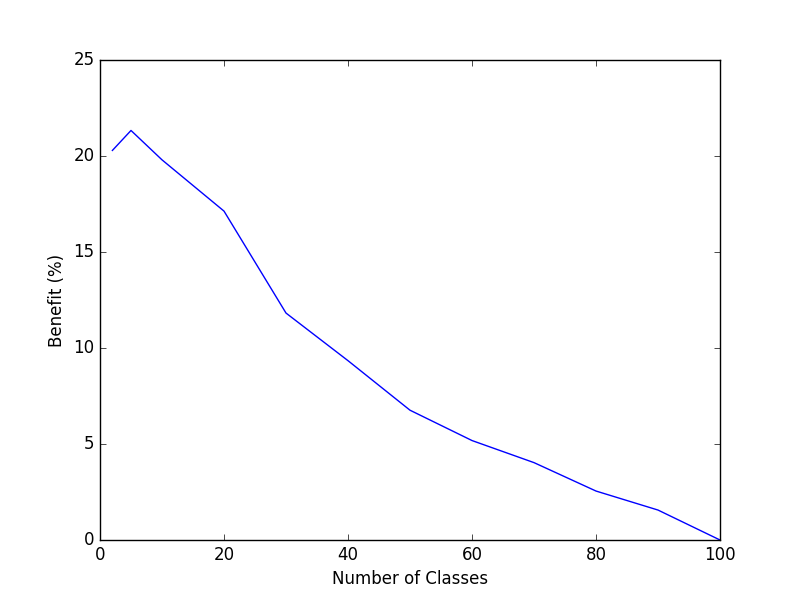
\includegraphics[scale=0.43]{figure_1.png}
\caption{Probability Layer Result}
\label{fig:ProbabilityLayer}
\end{figure}


\begin{table*}[!th]
    \centering
    \begin{tabular}{l|c|c|c}
        \hline
        \multicolumn{1}{c|}{Test Data} & Parameter  & Accuracy & Benefit \\
        Original CIFAR100 & 0 & 73.74\% &  \\
        \hline
        2 classes (0, 1) & 0 & 88.12\% &  \\
        2 classes (0, 1) & 1.0 & 98.51\% & +10.39\% \\
        \hline
        2 classes (3, 5) & 0 & 61.39\% &  \\
        2 classes (3, 5) & 1.0 & 99.01\% & +37.62\% \\
        \hline
        2 classes (0, 99) & 0 & 84.65\% & \\
        2 classes (0, 99) & 1.0 & 97.52\% & +12.87\% \\
        \hline
        5 classes $(0, ..., 4)$ & 0 & 66.33\% &  \\
        5 classes $(0, ..., 4)$ & 1.0 & 93.03\% & +26.70\% \\
        \hline
        5 classes $(5, ..., 9)$ & 0 & 81.06\% &  \\
        5 classes $(5, ..., 9)$ & 1.0 & 97.01\% & +15.95\% \\
        \hline
        10 classes $(0, ..., 9)$ & 0 & 75.35\% &  \\
        10 classes $(0, ..., 0)$ & 1.0 & 94.21\% & +18.86\% \\
        \hline
        10 classes $(10, ..., 19)$ & 0 & 67.16\% &  \\
        10 classes $(10, ..., 19)$ & 1.0 & 91.42\% & +24.26\% \\
        \hline
        10 classes $(20, ..., 29)$ & 0 & 75.84\% &  \\
        10 classes $(20, ..., 29)$ & 1.0 & 92.22\% & +16.38\% \\
        \hline
        
        
    \end{tabular}
    \vspace{1em}
    \caption{Test Probability Layer on Different Locality}
    \label{tab:ProbabilityLayer1}
\end{table*}



\subsubsection{Intuition and Shortcomings for probability layer}
The success of probability layer depends on the accuracy of original model. Intuitively, adding a constant to a set of domain classes according to the run-time distribution would encourage the model to select among these domain classes. If the original model is precise, i.e. have high top-5 accuracy, this constrain could rule out some classes and help the model to get a correct result. For example, if the output of softmax layer is $(0.3, 0, ..., 0, 0.7)$ and the probability layer according to runtime distribution is $(0.5, 0.5, 0.5, 0.5, 0.5, 0, ..., 0)$, the output of probability layer would be $(0.8, 0.5, 0.5, 0.5, 0.5, 0, ..., 0.7)$. Assume the correct label is $0$,  the prediction without probability layer is $99$, which is wrong, and the prediction with probability layer is $0$, which is correct. In this case, probability layer helps us to rule out the unlikely class $99$.

A possible case is that the probability corresponding to the true label are not highest even in domain classes. In this case, the probability will not be helpful. We found that top-5 accuracy is a good meric to measure how well the probability layer could help the original model. In other word, the benefit of probability layer is to improve the top-1 accuracy to be as large as the top-5 accuracy. If the top-5 accuracy is very high, the true label would have the top-5 high probability. The probability layer will constrain the predicted label to be the intersection between these top-5 labels and the domain labels according to runtime distribution. Thus we can increase top-1 accuracy toward top-5 accuracy. 

However, if the number of domain classes are 5 and the top-5 accuracy of the model is low, it is possible that the probability of true label is not the highest among the 5 domain classes. In this case, the benefit of probability layer would be slight. Thus, the higher top-5 accuracy the original model have, the better effect the probability layer would bring. In other word, if we use probability layer on a model with low top-5 accuracy, the benefit would be small. 

%The following is another scenario. Assume the true label is $0$ again. The output of softmax layer is $(0.3, 0.7, 0, 0, 0, ..., 0)$. After probability layer, the result is $(0.8, 1.2, 0.5, 0.5, 0.5, 0, ..., 0)$. In this scenario, the predicted result with and without probability layer both are 2, which are wrong. The probability layer cannot help because label $2$ is also in the domain classes $0$ to $4$. We believe that this case will not often happen from the perspective of probability for two reasons. First, according to the discussion in the last paragraph, we will use models that have high top-5 accuracy

\subsubsection{Comparison with naive mask}
A naive method is to mask all non-domain classes, called \textit{naive mask}. Probability layer is a generalization of naive mask. In fact, naive mask is equivalent to set the parameter $c$ in probability layer to be $1.0$. The intuitive explanation of naive mask is to only have nodes according to the main classes since the predicted label could only be one of these domain classes. If we use naive mask, all the prediction of images with classes besides the main classes would be wrong. This would limit the usage of naive mask dramatically. For example, if the domain classes occupy 70\% in the runtime distribution, the accuracy with naive mask would be less than 70\%, which is smaller than the accuracy without naive mask and makes naive mask useless, even if 70\% skew is not a low skew in daily life. 

Probability layer can avoid this problem if we set the parameter c to be strictly less than 1.0. This benefit depends on high accuracy of original model again. Generally, in denseNet, if an image could be classified correctly, the probability corresponding to the correct label after softmax layer is 1, and the probability corresponding to other labels are almost 0. For example, if the true label of an image is $11$, the output of softmax would generally be $(0, 0, 0, 0, 0, 0, 0, 0, 0, 0, 1, 0, 0, 0, 0, ... 0)$. Even if we add a probability layer to first 10 classes and use the parameter as 0.9, the output would be $(0.9, 0.9, 0.9, 0.9, 0.9, 0.9, 0.9, 0.9, 0.9, 0.9, 1, 0, 0, 0, 0, ... 0)$. In this case, the model would still mark $11$ as the correct label and the probability layer has no bad effect. However, if we use naive mask to rule out all classes other than first ten classes, the prediction would be constrained in the first ten classes and will be wrong. 

In other words, the probability layer only has bad effect when the original model is not quite sure about how to classify an image. For example, if the true label of an image is 11, the output might be $(0.3, 0, 0, 0, 0, 0, 0, 0, 0, 0, 0.7, 0, 0, 0, 0, ... 0)$. After we add the probability layer to first 10 classes and use the parameter as 0.9, the output would be $(1.2, 0.9, 0.9, 0.9, 0.9, 0.9, 0.9, 0.9, 0.9, 0.9, 0.7, 0, 0, 0, 0, ... 0)$. In this case, the model would mark 1 as the correct label and the probability layer have a bad effect. However, the happen of this bad effect needs two conditions. First, the labels with predicted probability 0.3 and 0.7 also appear in the first ten classes. Second, the predicted probability of true label is lower than the other one. Actually this is a rare case.

We have also done some experiments to support our result. Figure \ref{fig:NaiveMask} shows the comparison between probability layer and naive mask under different configurations. The red dash line represents the original accuracy without probability layer and naive mask, which is 74.57\%. When the number of domain classes is 10 and the distribution skew is 50\%, the accuracy with probability layer is 75.28\%, while the accuracy with naive mask is only 47.49\%. Thus probability layer has a positive effect even if the distribution skew is only 50\%, while the naive mask has a strong negative effect in this context. As we increase distribution skew gradually, the accuracy with probability layer and naive mask keeps increasing. Only after the distribution skew becomes larger than 77.67\%, naive mask starts to show positive effect on accuracy while probability layer keeps showing positive effect in all settings. As distribution skew approaches 100\%, the effect of naive mask catches probability layer up, since the true labels start to only exist in domain classes. In short, probability layer is a generalization of naive mask and shows benefit over original model and naive mask consistently.

\begin{figure}
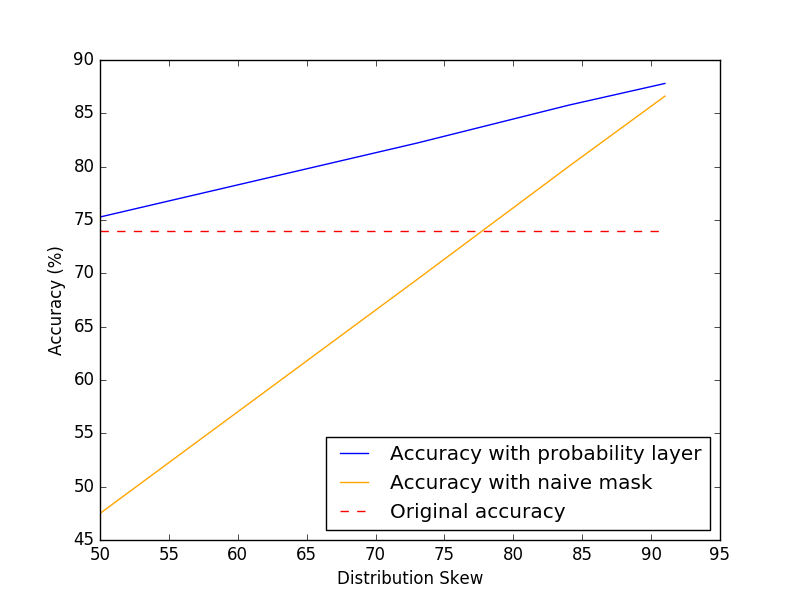
\includegraphics[scale=0.43]{figure_1-1.png}
\caption{Comparison Between Probability Layer and Naive Mask}
\label{fig:NaiveMask}
\end{figure}







\subsection{Old Content for probability layer}

Specialization says there are chances to make use of context information. The way to use this information is to re-train a specialized model. For this specialized model, we still assume all images appears with same frequency. This is kind of fixed. Actually, as we detect new images one by one, the probability distribution is changing gradually. In this process, \textit{how can we make use of the underlying distribution smoothly without re-training?}\textit{We want to find a formula which could make use of the existing knowledge about the distribution, while still leaving space for the underlying distribution to update.}

\subsubsection{Pre-knowledge}
Generic network aims for same frequency from all classes. However, if we have a knowledge about the frequency of different classes in our daily life, we can use this distribution as the underlying probability $P_{underlying}$ and use this information to adjust our prediction.


\subsubsection{Run-time Probability}
In run time, we can collect the probability distribution of various classes as $P(X)$. We can keep updating this underlying probability and use it to adjust our prediction.

\subsubsection{How can we implement Probability Layer}
In current DNNs for image classification, the last layer is always softmax layer
\begin{equation}
    y_i = \frac{exp(x_i)}{\sum_{j = 0}^{n}exp(x_j)}, i \in \{1,...,n\}
\end{equation} , where $x_i$ stands for the logits calculated from previous layers and n is the number of classes. Since the output $y_i$ would always be a number between $0$ and $1$, $y_i$ is seen as $P(X = i)$ and the class $i$ corresponding to the largest $y_i$ is chosen as the predicted class. A good method would be using the linear combination of softmax and underlying probability distribution 
\begin{equation}
P(X = i) = a \cdot softmax(X_i) + b \cdot P_{underlying}(X = i)    
\end{equation}
, where $a+b = 1$. We call this extra computation as the probability layer.

We should update $P_{underlying}$ after every prediction, using 
\begin{equation}
    P_{underlying}(X = j) = \frac{num(j)+  \mathbbm{1}\{i = j\} }{totalNum + 1}
\end{equation}
, where num(j) is the appearance number of class j in recent 30 minutes, totalNum is the number of images that has been processed in recent 30 minutes, and $\mathbbm{1}\{i = j\}$ is the indicator function such that
\begin{equation}
  \mathbbm{1}\{i = j\}=\begin{cases}
    1, & \text{if $i==j$}.\\
    0, & \text{otherwise}.
  \end{cases}
\end{equation}

\subsubsection{When should we implement Probability Layer}
We should always use probability layer as an additional one above the softmax layer. 


\section{Architecture}
In this section, we will describe the architecture in detail. Figure \ref{fig:Architecture} gives an overview of the architecture. Basically, we have 5 parts including two storage parts, class catalog and model store, one scheduler, one executor, and a profiler. The storage components, class catalog and model store, are used for saving metadata and providing supporting information for decision. The scheduler is a scheduling model to decide the choice of models in the runtime according to available resource and demanded accuracy. The target of the scheduler is to maximize the accuracy while adjust the energy consumption automatically according to remaining energy. The scheduler will also have a have high-accuracy mode just in case that users confront important scenario and want to get the best accuracy no matter how much energy the model will cost, or the user knows that a re-charge will be available soon. Once the scheduler made a decision, the executor will execute the model and the profiler will record the predicted value and update its record for future reference from the scheduler. Now we will discuss each component in detail.







\subsection{Profiler}
For every image, there would be a CNN model to classify it, either a full model or a specialized model. Thus every incoming image will have a predicted label. The profiler will record the distribution of classes and report the class skew to the scheduling model, which will use this information to choose the model. There would be two behaviors of profiler. First, the profiler will report the class skew every minute. Generally, the class skew would keep similar and change gradually as time goes and the class skew in current minute is a good approximation of the class skew in the following minute. And one minute is not a too short time period and hopefully a one-minute time window could see all the type of figures in current environment. This choice is a parameter instead of an unchangeable assumption. Second, after the profiler report the class skew to scheduler, it will still record the class skew. Through this way, the profiler can know, for this specific user, what kind of class skew will appear, how long the class skew will last, and how often this class skew will appear. This could be an important supporting information for the scheduler. If a class skew appears frequently, we can cold-retrain a complex model and save the model on disk. Once we see the class skew again, we can use this on-disk specialized model directly without retraining. Actually, it is quite common for a specific user that the same class skew appears everyday. For example, the people in family always remain same; the researchers will go to the lab everyday and the people in lab generally is changed once per year; the type and location of fitness equipments in a gym will also be same day by day. Once the profiler can detect this kind of class skew, the cold-retrain complex model could become a feasible choice.

\subsection{Class catalog}
When the profiler detect a class skew, we will consider not only the number of classes, but also the relationship between these classes. Class catalog is a tree-structured dictionary to group similar classes together. As we have discussed in section 2.2, if the detected class skew is close to each other in class catalog, it would be hard to classify these classes and the scheduler will use a more complex model to achieve the demanded accuracy. 


\subsection{Model Store}
In the beginning, there would be a collection of models without consideration on class skew. These models are for different purpose and with different degree of optimization. In the running time, as the profiler detect the class skew and usage pattern for the specific user, more specialized model, either hot retrained or cold retrained model, will be incorporated into the model store. When the device is connected to power and computation resource is enough, each model will be run on a benchmark, a collection of common datasets, like CIFAR100, and the average accuracy, energy and memory consumption will be recorded. In the run time, the scheduler can read this metadata from model store and use these information for decision. 

Another task that model store will accomplish automatically is to get the most efficient model for every energy budget. Given a energy budget, only the model with highest accuracy will be kept. In the same time, only the model with lowest resource consumption will be kept given a accuracy. This can be done by model store automatically since it is straightforward to calculate the number of parameter and computations just by going through a model without actually running. In this way, only the model that achieves Pareto optimality will be kept in model store and the scheduler can easily choose the most suitable model according to current energy budget just like a hash function.


\subsection{Scheduling Model}
The task of scheduling model is to select a series of models to process the image stream under a resource constrain. The target is to maximize the accuracy while try to use less energy for each image. The choice is between a cascades of models with different accuracy and different energy consumption. To solve this optimization problem, we build a heuristic algorithm, in Algorithm 1 and Algorithm 2 to allocate energy for each input image, choose the most suitable model given the per frame energy, and wrap all the decisions automatically.


Through a series of experiments (TO BE ADDED) on real-life videos, we found that the contents of a video would almost remain same in a single second, a process rate of one frame per second is enough for detect objects in the video. For energy efficiency consideration, we will use this configuration and estimate the per frame energy based on this observation. In concrete, $AllocateEnergy$ (line 11) will retrieve the expected running time and estimate per frame energy by averaging the available energy over all remaining time. In this case, saving energy in each frame still makes sense, since the saved energy will be allocated to future inputs and increase the accuracy of these inputs.

For giving more freedom to users, a $mode$ option is given through $scheduler$ (line 1) function. This option is useful if the user feel that current scenario is very important such that we want to sacrifice energy-efficiency for exchanging higher accuracy. In this case, the scheduler will expect to run for at least 10 minutes, no matter how long the original settled remaining time is, and allocate more energy to each frame. 



\begin{algorithm}
 \caption{Scheduling Model}
  \begin{algorithmic}[1]
    \Function{Scheduler}{$i, r, mode$}
        \Comment{i is the input image, r is the report from profiler about current class skew, mode is the user preference, target indicates the desired accuracy if mode is set to be EFFICIENCY}
        \State $AE = RemainEnergy()$    
        \Comment{AE stands for available energy}
        \If {mode == HIGHACCURACY}
            \State $PFE = AE / 600 $ 
            \Comment{PFE stands for perFrameEnergy, which is the energy allocated for every frame.}
        \ElsIf {mode == EFFICIENCY}
                \State $PFE = allocateEnergy(AE)$
        \EndIf
            \State $a, m = chooseModel(PFE, r)$  
                \Comment{chooseModel(PFE,r) is a function to access the metadata from class catalog and model store to decide the best accuracy we can achieve under current energy constrain and which model we should use}
            \State $execute(i,m)$        
                \Comment{execute(i,m) will retrieve the model m from model store and process the input image i with model m}
    \EndFunction

    \Function{allocateEnergy}{$AE$}
    \Comment{allocateEnergy(AE) allocates per frame energy according to current avalable energy and class skew}
        \State $n = RemainingTime()$    \Comment{remainingTime() will give the expected time to keep running. We will process one image per seconds and n is the remaining time in second as well as the expected number of images to classify.}
        \State $PFE = AE/n$
        \State \Return $PFE$
    \EndFunction
\end{algorithmic}
\end{algorithm}


Given per frame energy budget and recorded class skew, $ChooseModel$ will return the best model. If no class skew exists, $ChooseModel$ do not need to consider retraining and will choose the model with highest accuracy given current energy budget. When there is class skew, the $ExistedRetrainedModel$ will check whether there are retrained model for current class skew and return a suitable model. When there is no retrained model on disk, the architecture will choose between retraining last few layers and using probability layer. Since retraining is costly, we expect to have enough energy to run that retrained model for at least 10 minutes, otherwise it is more feasible to avoid retraining and use probability layer directly.


The scheduler will wrap up all the algorithms in scheduling model and give the most suitable model. For every input image $i$, The scheduler needs to get the class skew report $r$ from profiler. In the high accuracy mode, enough energy is given to each image such that more freedom in choice of models is allowed. In the efficiency mode, $allocateEnergy$ will estimate per frame energy according to expected remaining running time. Given this per frame energy and class skew report, the chooseModel will give the best model $m$ and the corresponding accuracy $a$. Finnaly, the $scheduler$ will call $execute(i,m)$ to run the model $m$ on input image $i$.

\begin{algorithm}
 \caption{Model Choice}
  \begin{algorithmic}[2]
    \Function{chooseModel}{$PFE, r$}
        \If{$Parse(r) == NoSkew$}
            \State $a, m = getModel(PFE)$   \Comment{If there is no class skew, getModel(PFE) will return the model with highest accuracy given the per frame energy budget PFE}
        \ElsIf{$Parse(r) == Skew$}
            \State $a,m = ExistedRetrainedModel(r, PFE)$
            \If{$m == NULL$}
                \If{$PFE > \Delta E/600 + FrameCost(m,r)$}
                    \State $a,m = retrain(m,r)$
                \Else
                    \State $a,m = probabilityLayer(m,r)$
                \EndIf
            \EndIf
        \EndIf
        
        \State \Return $a,m$
    \EndFunction
    

\end{algorithmic}
\end{algorithm}




\section{Experiments}
\subsection{Effectiveness of specialization}

\subsection{Effectiveness of distillation}

\subsection{Effectiveness of pre-knowledge}

\subsection{Effectiveness of run-time probability}

\section{Comparison with previous work}
\subsection{Specialization}


\subsection{Distillation}
Model Compression \cite{bucilu2006model} trains ensembles of neural network on the original dataset, and uses these ensembles to label a large unlabeled dataset. Instead of training the neural network on the original training dataset, Model Compression would train the neural network on this much larger, ensemble labeled dataset. This neural network can perform much better than a neural network with the same structure but trained only using the original dataset.

Deeper network tends to perform better than shallow ones and have stronger ability in abstracting information from datasets. Instead of training shallow network only using original datasets, Distillation \cite{hinton2015distilling} shows that we can train them to mimic the logits of deep networks.

The most common method to achieve high energy efficiency is to reduce the size of network. FitNet \cite{romero2014fitnets} uses deepper but thinner networks to mimic the original model, through which FitNet can use less parameters and computation to achieve similar accuracy compared with the original model.

MCDNN \cite{han2016mcdnn} Used a series of compression and specialization to generate sequence of variants of the original model, which generates the trade between accuracy and memory/energy. Then MCDNN uses an optimization model to choose variants according to current energy and memory budgets.



\section{Conclusion and Future Work}
By using runtime class skew, including reduction in number of classes and similarity between a cluster of classes, we can increase accuracy without any change in model architecture. This phenonmenon gives us space to dramatically simplify our CNN models by changing input size, reducing number of nodes in softmax layer, reducing number of layers, and distillation.  Further, we can use probability layer to make use of this class skew without retraining if the energy budget is limited, or retrain the last few layers if energy constraint is loose. By recording the repeated pattern of classes, cold retrain the model is a feasible way to make use of runtime distribution without runtime retrain. Finnaly, the end-to-end runtime support framework, SMART, can reduce energy consumption by xx times while increase the accuracy by xx times. (EXPERIMENTS TO BE ADDED). In the future, we will provide a more detailed mapping from class cluster to suggested models.

%% Structure:
%% 1.25 page for introduction
%% 0.75 page for related work
%% 2.5 pages for model description
%% 2 pages for experiments, including design and results
%% 0.5 page for conclusion and future work





%% The file named.bst is a bibliography style file for BibTeX 0.99c
\bibliographystyle{named}
\bibliography{sd}

\end{document}